\documentclass[12pt]{article}

\usepackage{tikz} 
\usepackage{amsmath}
\usepackage{color} 
 
\usetikzlibrary {math}

\begin{document}
    \title{El Problema CShaassandLights}
    \author{Daniel de la Cruz Prieto}
    \date{\today}

    \maketitle 

    % \section*{Orden del Problema}

    % \section*{In Inglish:}

    % \begin{flushleft}
    %     There are n lights aligned in a row. These lights are numbered 1 to n from left to right. Initially some of the lights are switched on. Shaass wants to switch all the lights on. At each step he can switch a light on (this light should be switched off at that moment) if there's at least one -adjacent light which is already switched on. 
    % \end{flushleft}
    % \begin{flushleft}
    %     He knows the initial state of lights and he's wondering how many different ways there exist to switch all the lights on. Please find the required number of ways modulo 1000000007 (109 + 7).
    % \end{flushleft}

    % \subsection*{Input}

    % \begin{flushleft}
    %     The first line of the input contains two integers n and m where n is the number of lights in the sequence and m is the number of lights which are initially switched on, (1 ≤ n ≤ 1000, 1 ≤ m ≤ n). The second line contains m distinct integers, each between 1 to n inclusive, denoting the indices of lights which are initially switched on.
    % \end{flushleft}

    % \subsection*{Output}

    % \begin{flushleft}
    %     In the only line of the output print the number of different possible ways to switch on all the lights modulo 1000000007 (109 + 7).
    % \end{flushleft}
    
    % \section*{En Espanol:}
    
    % \subsection*{Entrada}
    % \begin{flushleft}
    %     Hay n luces alineadas en una fila. Estas luces están numeradas del 1 al n de izquierda a derecha. Inicialmente, algunas de las luces están encendidas. Shaass quiere encender todas las luces. A cada paso, puede encender una luz (esta luz debe estar apagada en ese momento) si hay al menos una luz adyacente que ya está encendida.
    % \end{flushleft}

    % \subsection*{Salida}
    % \begin{flushleft}
    %     Conoce el estado inicial de las luces y se pregunta cuántas formas diferentes existen de encender todas las luces. Encuentre el número requerido de vías módulo 1000000007 (109 + 7).
    % \end{flushleft}
    % \begin{flushleft}
    %     La primera línea de la entrada contiene dos números enteros nym donde n es el número de luces en la secuencia y m es el número de luces que se encienden inicialmente, (1 ≤ n ≤ 1000, 1 ≤ m ≤ n). La segunda línea contiene m enteros distintos, cada uno entre 1 a n inclusive, que denota los índices de luces que se encienden inicialmente.
    % \end{flushleft}
    % \begin{flushleft}
    %     En la única línea de la salida imprima el número de diferentes formas posibles de encender todas las luces módulo 1000000007 (109 + 7).
    % \end{flushleft}
    
    % \section*{Example 1: (ejempo)}
    
    
    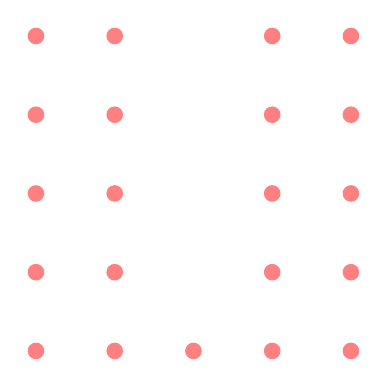
\begin{tikzpicture}
        \foreach \x in {0,...,4}
        \foreach \y in {0,...,4}
        {
            \ifnum \x=2
            \breakforeach
            \fi

            
            
            \fill[red!50] (\x,\y) ellipse (3pt and 3pt) ;

            
        }

        
    \end{tikzpicture}

\end{document}
